\documentclass{article}

\usepackage{fancyhdr}
\usepackage{extramarks}
\usepackage{boondox-cal}
\usepackage{amsmath}
\usepackage{amsthm}
\usepackage{amsfonts}
\usepackage{tikz}
\usepackage[plain]{algorithm}
\usepackage{algpseudocode}

\usetikzlibrary{automata,positioning, arrows.meta}

%
% Basic Document Settings
%

\topmargin=-0.45in
\evensidemargin=0in
\oddsidemargin=0in
\textwidth=6.5in
\textheight=9.0in
\headsep=0.25in

\linespread{1.1}

\pagestyle{fancy}
\lhead{\hmwkAuthorName}
\chead{\hmwkClass\ (\hmwkClassInstructor): \hmwkTitle}
\rhead{\firstxmark}
\lfoot{\lastxmark}
\cfoot{\thepage}

\renewcommand\headrulewidth{0.4pt}
\renewcommand\footrulewidth{0.4pt}

\setlength\parindent{0pt}

%
% Create Problem Sections
%

\newcommand{\enterProblemHeader}[1]{
    \nobreak\extramarks{}{Problem \arabic{#1} continued on next page\ldots}\nobreak{}
    \nobreak\extramarks{Problem \arabic{#1} (continued)}{Problem \arabic{#1} continued on next page\ldots}\nobreak{}
}

\newcommand{\exitProblemHeader}[1]{
    \nobreak\extramarks{Problem \arabic{#1} (continued)}{Problem \arabic{#1} continued on next page\ldots}\nobreak{}
    \stepcounter{#1}
    \nobreak\extramarks{Problem \arabic{#1}}{}\nobreak{}
}

\setcounter{secnumdepth}{0}
\newcounter{partCounter}
\newcounter{homeworkProblemCounter}
\setcounter{homeworkProblemCounter}{1}
\nobreak\extramarks{Problem \arabic{homeworkProblemCounter}}{}\nobreak{}

%
% Homework Problem Environment
%
% This environment takes an optional argument. When given, it will adjust the
% problem counter. This is useful for when the problems given for your
% assignment aren't sequential. See the last 3 problems of this template for an
% example.
%
\newenvironment{homeworkProblem}[1][-1]{
    \ifnum#1>0
        \setcounter{homeworkProblemCounter}{#1}
    \fi
    \section{Problem \arabic{homeworkProblemCounter}}
    \setcounter{partCounter}{1}
    \enterProblemHeader{homeworkProblemCounter}
}{
    \exitProblemHeader{homeworkProblemCounter}
}

%
% Homework Details
%   - Title
%   - Due date
%   - Class
%   - Section/Time
%   - Instructor
%   - Author
%

\newcommand{\hmwkTitle}{Homework\ \#4}
\newcommand{\hmwkDueDate}{February 28, 2024}
\newcommand{\hmwkClass}{Linear Algebra}
\newcommand{\hmwkClassInstructor}{Gilbert Strang}
\newcommand{\hmwkAuthorName}{\textbf{0130}}

%
% Title Page
%

\title{
    \vspace{2in}
    \textmd{\textbf{\hmwkClass:\ \hmwkTitle}}\\
    \vspace{0.1in}\large{\textit{\hmwkClassInstructor}}
    \vspace{3in}
}

\author{\hmwkAuthorName}
\date{}

\renewcommand{\part}[1]{\textbf{\large Part \Alph{partCounter}}\stepcounter{partCounter}\\}

%
% Various Helper Commands
%

% Useful for algorithms
\newcommand{\alg}[1]{\textsc{\bfseries \footnotesize #1}}

% For derivatives
\newcommand{\deriv}[1]{\frac{\mathrm{d}}{\mathrm{d}x} (#1)}

% For partial derivatives
\newcommand{\pderiv}[2]{\frac{\partial}{\partial #1} (#2)}

% Integral dx
\newcommand{\dx}{\mathrm{d}x}

% Alias for the Solution section header
\newcommand{\solution}{\textbf{\large Solution}}

% Probability commands: Expectation, Variance, Covariance, Bias
\newcommand{\E}{\mathrm{E}}
\newcommand{\Var}{\mathrm{Var}}
\newcommand{\Cov}{\mathrm{Cov}}
\newcommand{\Bias}{\mathrm{Bias}}

% empty underline
\newcommand{\emptyunderline}{\underline{\ \ \ \ \ \ }}

\begin{document}

\maketitle

\pagebreak

Since in this homework we repeatedly use the fact that if the columns of \( A \)
is linearly independent then we have the matrix \( A^T A \) is invertible, I want to
prove this at the beginning.
\\

So the core is that I want to show that \( x \) must be \( \mathbf{0} \) if the columns
of \( A \) is independent and \( A^T A x = 0 \), the method in lecture 16 is that we can
multiply the transpose of \( x \) in the both sides of the equation, then we get \( x^T A^T A x = {(Ax)}^T (Ax) = 0 \),
then we know \( Ax = 0 \). But we can also think of that since the columns of \( A \) is independent, we have
\( \dim {\mathbf{N}(A^T)} = 0 \), which means \( Ax \) must be the zero vector. Then using the 
assumption of the independency of columns, we know \( x \) must be the zero vector.

\begin{homeworkProblem}

    Find the \textbf{incidentce matrix} and its rank and one
    vector in each subspace for this complete graph---all six
    edges included.
    
    \[
    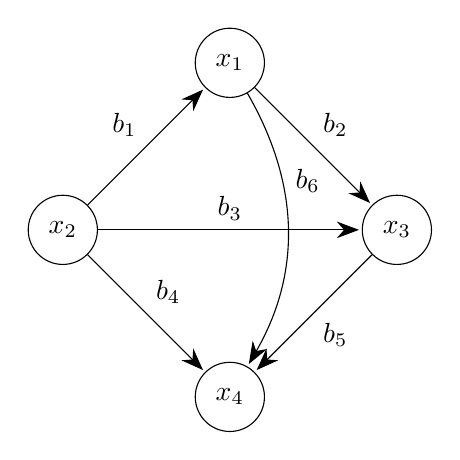
\begin{tikzpicture}[>={Stealth[length=8pt]}, shorten >= 1pt, node distance = 3cm, on grid, auto]
        \node[state] (x2) {$x_2$};
        \node[state] (x1) [above right=of x2] {$x_1$};
        \node[state] (x4) [below right = of x2] {$x_4$};
        \node[state] (x3) [above right=of x4] {$x_3$};
        \path[->]
        (x2) edge node {$b_1$} (x1)
        (x1) edge node {$b_2$} (x3)
        (x2) edge node {$b_3$} (x3)
        (x2) edge node {$b_4$} (x4)
        (x3) edge node {$b_5$} (x4)
        (x1) edge [bend left] node[pos = 0.4, above right] {$b_6$} (x4)
        ;
    \end{tikzpicture}
    \]

    \solution

    \[
        \begin{bmatrix}
            -1 & 1 & 0 & 0  \\
            -1 & 0 & 1 & 0  \\
            0 & -1 & 1 & 0  \\
            0 & -1 & 0 & 1  \\
            0 & 0 & -1 & 1  \\
            -1 & 0 & 0 & 1
        \end{bmatrix}
    \]

\end{homeworkProblem}

\begin{homeworkProblem}
    \textbf{If} \( \mathbf{A^T A x = 0} \) \textbf{then} \( \mathbf{Ax = 0} \).
    Reason: \( A\mathbf{x} \) is in nullspace of \( A^T \) and
    also in the \emptyunderline\ of \( A \) and those spaces are \emptyunderline. 
    Conclusion: \( A\mathbf{x = 0} \) and therefore\( A^T A \)
    has the same nullspace as \( A \). This key fact will be repeated when we need it.
    \\

    \solution

    \begin{enumerate}
        \item Column space.
        \item Orthogonal.
    \end{enumerate}
\end{homeworkProblem}

\begin{homeworkProblem}
    Compute the projection matrices \( \mathbf{a} \mathbf{a}^T / \mathbf{a}^T \mathbf{a} \)
    onto lines through \( \mathbf{a}_1 = (-1, 2, 2) \) and \( \mathbf{a}_2 = (2, 2, -1) \).
    Multiply those projection matrices and explain why their product \( P_1P_2 \) is what it is.
    \\

    \solution

    \[
        P_1 = \begin{bmatrix}
            1 & -2 & -2 \\
            -2 & 4 & 4 \\
            -2 & 4 & 4
        \end{bmatrix}
        ,
        P_2 = \begin{bmatrix}
            4 & 4 & -2 \\
            4 & 4 & -2 \\
            -2 & -2 & 1
        \end{bmatrix}
        ,
        P_1P_2 = \begin{bmatrix}
            0 & 0 & 0 \\
            0 & 0 & 0 \\
            0 & 0 & 0
        \end{bmatrix}
    \]
    \\

    The product \( P_1P_2 \) is the zero matrix because the lines through \( \mathbf{a}_1 \) and \( \mathbf{a}_2 \) are orthogonal.

\end{homeworkProblem}

\begin{homeworkProblem}
    Suppose \( A \) is the 4 by 4 identity matrix with its last column
    removed. \( A \) is 4 by 3. Project \( \mathbf{b} = (1, 2, 3, 4) \)
    onto the column space of \( A \). What shape is the projection matrix
    \( P \) and what is \( P \)?
    \\

    \solution
    \begin{enumerate}
        \item The shape of matrix \( P \) is 4 by 4.
        \item The columns of \( A \) is a basis
            of the column space of \( A \). Let \( \mathbf{p} \) represents the projection of
            \( \mathbf{b} \), then error can be represented as \( \mathbf{e = b - p} \), and we
            know \( C(A) \) and \( \mathbf{e} \) are orthogonal so \( \mathbf{e} \in \mathbf{N}(A^T) \)
            therefore \( A^T \mathbf{e} = 0 \). Since \( \mathbf{p} \) is in the column space of \( A \),
            \( \mathbf{p} \) can be represented as a linear combination of the columns of \( A \), therefore
            \( \mathbf{p} \) can be written as \( \mathbf{p} = A \mathbf{\hat{x}} \), and we have:

            \[
                P = A{(A^T A)}^{-1}A^T = \begin{bmatrix}
                    1 & 0 & 0 & 0   \\
                    0 & 1 & 0 & 0   \\
                    0 & 0 & 1 & 0   \\
                    0 & 0 & 0 & 0
                \end{bmatrix}
            \]
    \end{enumerate}
    
\end{homeworkProblem}

\begin{homeworkProblem}
    What linear combination of (1, 2, -1) and (1, 0, 1) is closest
    to \( \mathbf{b} = (2, 1, 1) \)?
    \\

    \solution
    \\

    Similar to Problem 4, let \( \mathbf{e, p} \) represent error and the projection
    of \( \mathbf{b} \) seperately, and use \( \mathbf{\hat{x}} \) represents the coeffcients
    of the cloest linear combination, we have 
    \[ 
        \mathbf{\hat{x}} = {(A^T A)}^{-1} A^T \mathbf{b} 
        = \begin{bmatrix}
            1 / 3 \\
            3 / 2
        \end{bmatrix}
    \]

    so the cloest linear combination of \( \mathbf{b} \) is \( \frac{1}{3} \begin{bmatrix}
        1&   \\
        2&   \\
        -1&  \\
    \end{bmatrix} + \frac{3}{2}
    \begin{bmatrix}
        1   \\
        0   \\
        1
    \end{bmatrix}
    \).
\end{homeworkProblem}

\begin{homeworkProblem}
    To find the projection matrix onto the plane \( x - y - 2z = 0 \), 
    choose two vectors in that plane and make them the columns of \( A \).
    The plane will be the column space of \( A \)! Then compute \( P = A {(A^T A)}^{-1} A^T \).

    \[ \mathbf{OR} \]

    To find the projection matrix \( P \) onto the same plane \( x - y - 2z = 0 \),
    write down a vector \( \mathbf{e} \) that is perpendicular to the plane. Compute the projection
    \( Q = \mathbf{e e^T}/\mathbf{e^T e}\) and then \( P = I - Q \).
    \\

    \solution
    \\

    \begin{enumerate}
        \item First method. Choose \( \mathbf{v}_1 = \begin{bmatrix}
            1 & 1 & 0
        \end{bmatrix} \) and \( \mathbf{v}_2 = \begin{bmatrix}
            0 & 2 & -1
        \end{bmatrix} \) as a basis of the plane. Let \( A = \begin{bmatrix}
            1 & 0   \\
            1 & 2   \\
            0 & -1
        \end{bmatrix} \), then compute projection matrix 
        \[ P = A {(A^T A)}^{-1} A^T = \begin{bmatrix}
            5 / 6 & 1 / 6 & 1 / 3   \\
            1 / 6 & 5 / 6 & - 1 / 3  \\
            1/ 3 & - 1 / 3 & 1 / 3
        \end{bmatrix}
        \]
    \item Second method. We can pick the coeffcients of the plane equation as a vector
        which is perpendicular to to the plane, this is because for a plane equation, we can think
        of it as being the dot product of two vectors, one of which is an arbitrary vector in the 
        plane \( (x, y, z) \) while the other is a vector perpendicular to the plane. So \( \mathbf{e} = (1, -1, -2) \).
        Since a vector \( \mathbf{b} \) can be represented as two part \( \mathbf{p'} + \mathbf{e'} \) where \( \mathbf{p'} \in 
        C(A) \) and \( \mathbf{e'} \in \mathbf{N}(A^T) \), therefore \( P\mathbf{b} = \mathbf{b} - Q\mathbf{b} \), where \( Q \) is
        the projection matrix of \( \mathbf{b} \) onto \( \mathbf{e} \), and we all know the formula of \( Q \) is 
        \[ 
            Q = \mathbf{e e^T} / \mathbf{e^T e}  = \begin{bmatrix}
                1 / 6 & - 1 / 6 & - 1 / 3   \\
                - 1 / 6 & 1 / 6 & 1 / 3 \\
                - 1 / 3 & 1 / 3 & 2 / 3
            \end{bmatrix},
            P = I - Q = \begin{bmatrix}
                5 / 6 & 1 / 6 & 1 / 3   \\
                1 / 6 & 5 / 6 & - 1 / 3  \\
                1/ 3 & - 1 / 3 & 1 / 3
            \end{bmatrix}
        \]
    \end{enumerate}
\end{homeworkProblem}

\begin{homeworkProblem}
    The first three Chebyshev polynomials are given by
    
    \( T_0(x) = 1,\ \ T_1(x) = x,\ \ T_2(x) = 2x^2 - 1 \)

    \begin{enumerate}
        \item Show that \( \left\{ T_0, T_1, T_2 \right\}\) is a basis for \( \mathbb{P}_2 \),
            the space of polynomials of degree \( \leq \) 2 (more generally, the space of polynomials
            of degree \( \leq \) n is denoted by \( \mathbb{P}_n \)).
        \item Check that differentiation defines a linear transformation \( T_D : \mathbb{P}_2 \to \mathbb{P}_1 \)
            and write down the matrix of each linear transformation in the Chebyshev basis. Similarly, check that
            integration is a linear transformation \( T_S = \mathbb{P}_1 \to \mathbb{P}_2 \).
        \item  Let \( D \) and \( S \) be the differentiation and integration matrices from part{(b)}. 
        Compute the matrix product \( DS \) and \( SD \). Interpret the results using calculus: choose
        a suitable polynomial in \( \mathbb{P}_2 \), differentiate it and then integrate it.
        \item Write down bases for the null spaces and column spaces of \( D \) and \( S \). Provide the
        corresponding polynomials. Can you interpret your results about \( D \) and \( S \) in light of what
        you know about differentiation and integration in calculus?
    \end{enumerate}

    \solution
    \\
    
    Let the entries of column represents the coeffcients of \( 1, x, x^2, \ldots \) from top to bottom,
    and \( \mathbf{v}_i \) represents the vector of \( T_i \).

    \begin{enumerate}
        \item The matrix of \(\left\{ T_0, T_1, T_2 \right\} \) is \( \begin{bmatrix}
            1 & 0 & -1  \\
            0 & 1 & 0   \\
            0 & 0 & 2
        \end{bmatrix} \),
        and its rank equals to 3. Since the a natural basis of \( \mathbb{P}_2 \) is \( \left\{ 1, x, x^2 \right\} \) which implies
        the dimension of this space is 3, we know \(\left\{ T_0, T_1, T_2 \right\} \) is a basis of \( \mathbb{P}_2 \).
        \item \begin{enumerate}
            \item Differentiation. 
                \[ 
                    \begin{split}
                        \frac{d}{dx}& \left\{ (a_1x^2 + b_1x + c_1)  + (a_2x^2 + b_2x + c_2)\right\}   \\
                        &= 2a_1x + b_1 + 2a_2x + b_2    \\
                        &= 2(a_1 + a_2)x + (b_1 + b_2)  \\
                        &= \frac{d}{dx}(a_1x^2 + b_1x + c_1) + \frac{d}{dx}(a_2x^2 + b_2x + c_2)
                    \end{split}
                \]
                The process above shows that differentiation is a linear transformation. The matrix of each 
                linear transformation in the Chebyshev basis is shown below:
                \[
                    \begin{bmatrix}
                        0 & 1 & 0   \\
                        0 & 0 & 2   \\
                    \end{bmatrix}
                \]
            \item Integration.
                    The process of checking that integretion is a linear transform is similar to the process above
                    and we omit the details here. The matrix of each linear transformation in the Chebyshev basis is shown below:

                    \[
                        \begin{bmatrix}
                            a & b & c    \\
                            1 & 0 & 0   \\
                            0 & 1 / 2 & 0   \\
                            0 & 0 & 1 /3 
                        \end{bmatrix}:
                        a, b, c \in \mathbb{R}
                    \]
        \end{enumerate}
        \item \begin{enumerate}
            \item Consider the matrix product \( DS \), the important thing is that, here the differentiation if a
                linear transformation from \( \mathbb{P}_3 \to \mathbb{P}_2 \), so the corresponding matrix is
                \[
                    \begin{bmatrix}
                    0 & 1 & 0 & 0   \\
                    0 & 0 & 2 & 0   \\
                    0 & 0 & 0 & 3
                    \end{bmatrix}
                \]
                what we need to know additionally is that \( T_3 = 4x^3 - 3x \),
                then we can compute the product \( DS \) as

                \[
                    DS = \begin{bmatrix}
                        1 & 0 & 0  \\
                        0 & 1 & 0   \\
                        0 & 0 & 1
                    \end{bmatrix}
                \]
    \item Consider the matrix product SD, similarly, we should notice that here the
        integration is a linear transformation from \( \mathbb{P}_1 \to \mathbb{P}_2 \), so the corresponding matrix is

        \[
            \begin{bmatrix}
                a & b  \\
                1 & 0   \\
                0 & 1/2
            \end{bmatrix}:
            a, b \in \mathbb{R}
        \]

        and we can compute the product \( SD \) as

        \[
            SD = \begin{bmatrix}
                0 & a & b  \\
                0 & 1 & 0 \\
                0 & 0 & 1
            \end{bmatrix}: a, b \in \mathbb{R}
        \]
    \end{enumerate}
    This is very interesting, as we know in calculus, in we do the differentiation after
    the integration, we can preserve all the information. But if we do the differentiation before
    the integration, we will lose the information of the contant order number. For example, we apply
    differentiation and then integration to \( x - 1 \), we have

    \[
        \int \frac{d}{dx}(x - 1)dx = \int 1dx = x + c, c \in \mathbb{R}
    \]

    but if we do the integration and then differentiation to \( x - 1 \), we have

    \[
        \frac{d}{dx}\int (x - 1)dx = \frac{d}{dx}(\frac{x^2}{2} - x) = x - 1
    \]

    \item 
        \begin{enumerate}
            \item 
    A basis of nullspace of \( D \) is \(
            \begin{bmatrix}
                1   \\
                0   \\
                0   \\
            \end{bmatrix}
        \)
        and the corresponding polynomials is the constant 1.
    \item A basis of column space of \( D \) is \( \left\{ \begin{bmatrix}
            1   \\
            0   \\
        \end{bmatrix}
        ,
        \begin{bmatrix}
            0   \\
            1
        \end{bmatrix}
        \right\}
        \), the corresponding polynomials is \( 1 \) and \( x \).
    \item A basis of nullspace of \( S \) is \( \left\{ \mathbf{0} \right\} \), there is no corresponding polynomial.
    \item A basis of column space of \( S \) is \( \left\{ 
        \begin{bmatrix}
        1   \\
        0   \\
        0   \\
        0
        \end{bmatrix},
     \begin{bmatrix}
        0   \\
        1   \\
        0   \\
        0
    \end{bmatrix},
     \begin{bmatrix}
        0   \\
        0   \\
        1   \\
        0
    \end{bmatrix},
     \begin{bmatrix}
        0   \\
        0   \\
        0   \\
        1
    \end{bmatrix}
    \right\} \),
    the corresponding polynomials is \( 1, x, x^2, x^3 \).
        \end{enumerate}
\end{enumerate}

These results can be interpreted using calculus. (a) is because
the constant is the only polynomial that has a derivative of 0, and (b) is because the whole
space of \( \mathbb{P}_1 \) is spanned by \( \left\{ 1, x \right\} \), (c) is result of the fact that
there does not exist any polynomial whose integral is zero polynomial and finally (d) is reasonable because
any polynomial with order \( \geq 0 \) (not zero polynomial) can be obtained by the integration of
a polynomial with order lower than it.


\end{homeworkProblem}

\end{document}